\subsection{Valuación de Opciones. Método del Arbol Binomial.}

Construir un árbol binomial es una técnica muy útil y popular para valuar opciones.  Un \textcolor{principal}{Arbol Binomial} es un diagrama que representa diferentes ``caminos'' que puede seguir el precio de un activo subyacente durante la vida de una opción.\\

El método está basado en la hipótesis de que el precio del activo subyacente se puede modelar como un \textcolor{principal}{Paseo Aleatorio}. En cada paso de dicho paseo ($\Delta t$, existe cierta posibilidad $p$ de que el precio de la opción aumente en una proporción $u$, o baje en una proporción $d$. Estos parámetros no dependen del precio del activo subyacente, si no que dependen del precio promedio y la volatilidad.\\
\begin{figure}[H]
\centering
\caption{Arbol Binomial de un paso.}
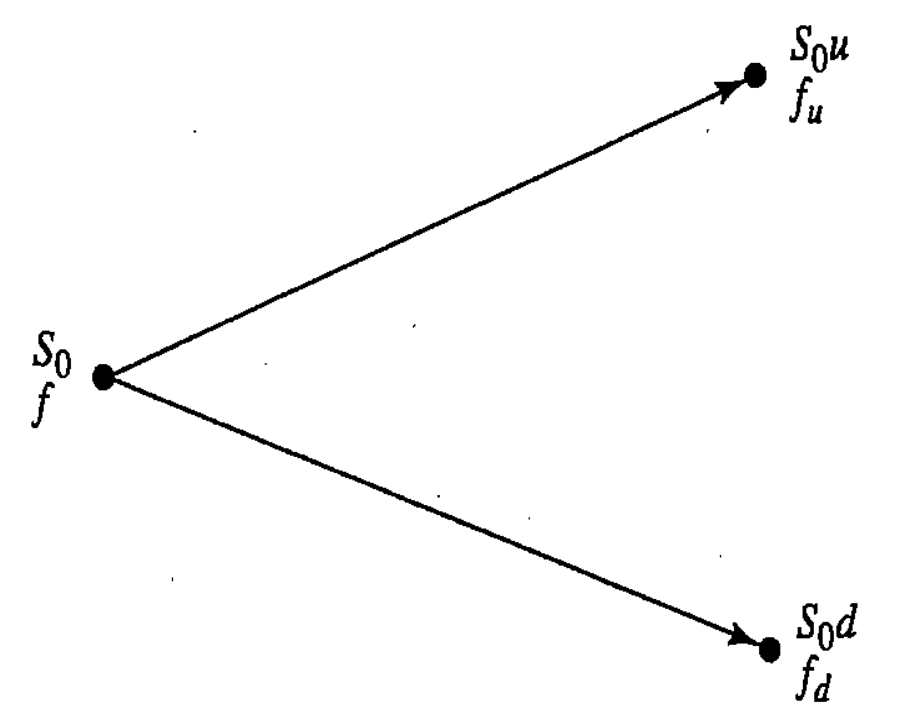
\includegraphics[width=8cm]{\rutaImagenes/arbol_binomial_1}
\end{figure}

En la figura anterior, $f=S_0$ es el precio Spot del activo subyacente, $f_u=S_0u$ es el precio del activo si es que éste aumenta y $f_d=S_0d$ es el precio del activo en caso de que disminuya.\\

Para elaborar un árbol binomial de más pasos, se itera el proceso tomando cada nuevo precio (Nodo) como precio Spot y se calculan los siguientes precios.\\

\begin{figure}[H]
\centering
\caption{Arbol Binomial de dos paso.}
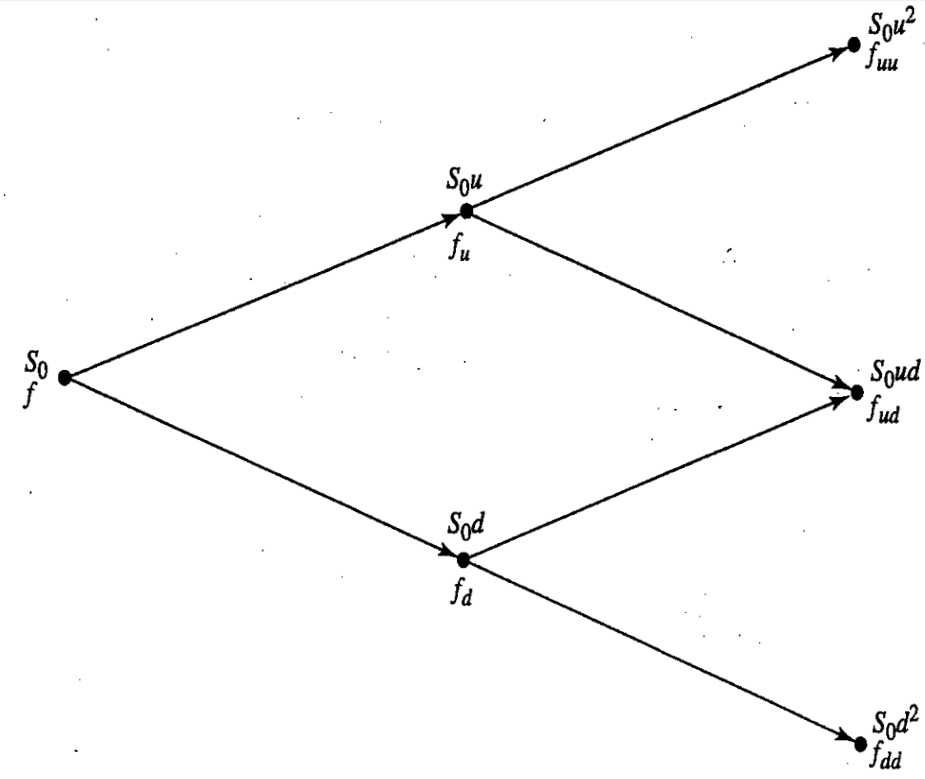
\includegraphics[width=8cm]{\rutaImagenes/arbol_binomial_2}
\end{figure}

